\documentclass[border=8pt,tikz]{standalone}
\usepackage{tikz}
% Shared TikZ style for Chapter 5 diagrams.
% Inputted by every standalone diagram file.

\usetikzlibrary{
  arrows.meta,
  positioning,
  shapes.geometric,
  shapes.symbols,
  shapes.multipart,
  shapes.misc,
  fit,
  calc,
  backgrounds,
  decorations.pathmorphing,
  decorations.pathreplacing,
  patterns,
  shadows.blur,
}

% ─── Colour palette ──────────────────────────────────────────────
\definecolor{strixBlue}{HTML}{3B7DD8}     % data sources / inputs
\definecolor{strixGreen}{HTML}{22A699}    % processing / workers
\definecolor{strixOrange}{HTML}{E08036}   % storage
\definecolor{strixRed}{HTML}{E04B4B}      % attacker / external threat
\definecolor{strixPurple}{HTML}{6B5DD3}   % frontend / UI
\definecolor{strixGold}{HTML}{F2BE22}     % models / ML
\definecolor{strixGrey}{HTML}{6E7681}     % neutral / labels
\definecolor{strixDark}{HTML}{1F2933}     % titles / borders

% ─── Common node styles ──────────────────────────────────────────
\tikzset{
  >={Latex[width=2mm,length=2.5mm]},
  font=\sffamily\small,
  every node/.style={align=center},
  comp/.style={
    rectangle, rounded corners=2pt, draw=#1, fill=#1!10, very thick,
    text=strixDark, minimum width=22mm, minimum height=8mm,
    inner sep=4pt,
  },
  comp/.default=strixGreen,
  store/.style={
    cylinder, shape border rotate=90, aspect=0.3, draw=strixOrange,
    fill=strixOrange!12, very thick, text=strixDark,
    minimum width=18mm, minimum height=10mm, inner sep=2pt,
  },
  stream/.style={
    rectangle, rounded corners=2pt, draw=strixOrange,
    fill=strixOrange!8, dashed, thick, text=strixDark,
    minimum width=22mm, minimum height=7mm, inner sep=3pt,
    font=\ttfamily\scriptsize,
  },
  source/.style={comp=strixBlue},
  worker/.style={comp=strixGreen},
  model/.style={comp=strixGold},
  ui/.style={comp=strixPurple},
  ext/.style={comp=strixRed},
  title/.style={font=\sffamily\bfseries, text=strixDark},
  edge/.style={->, thick, draw=strixGrey, font=\sffamily\scriptsize\itshape},
  edgeStrong/.style={->, very thick, draw=strixDark, font=\sffamily\scriptsize\bfseries},
  group/.style={
    rectangle, rounded corners=4pt, draw=strixGrey, dashed, thick,
    inner sep=6pt, fill=strixGrey!4,
  },
  badge/.style={
    rectangle, rounded corners=1pt, fill=#1, text=white,
    font=\sffamily\scriptsize\bfseries, inner sep=2pt,
  },
  badge/.default=strixDark,
  port/.style={
    rectangle, rounded corners=1pt, draw=strixDark, fill=strixGrey!8,
    font=\ttfamily\scriptsize, minimum width=14mm, inner sep=2pt,
  },
}


\begin{document}
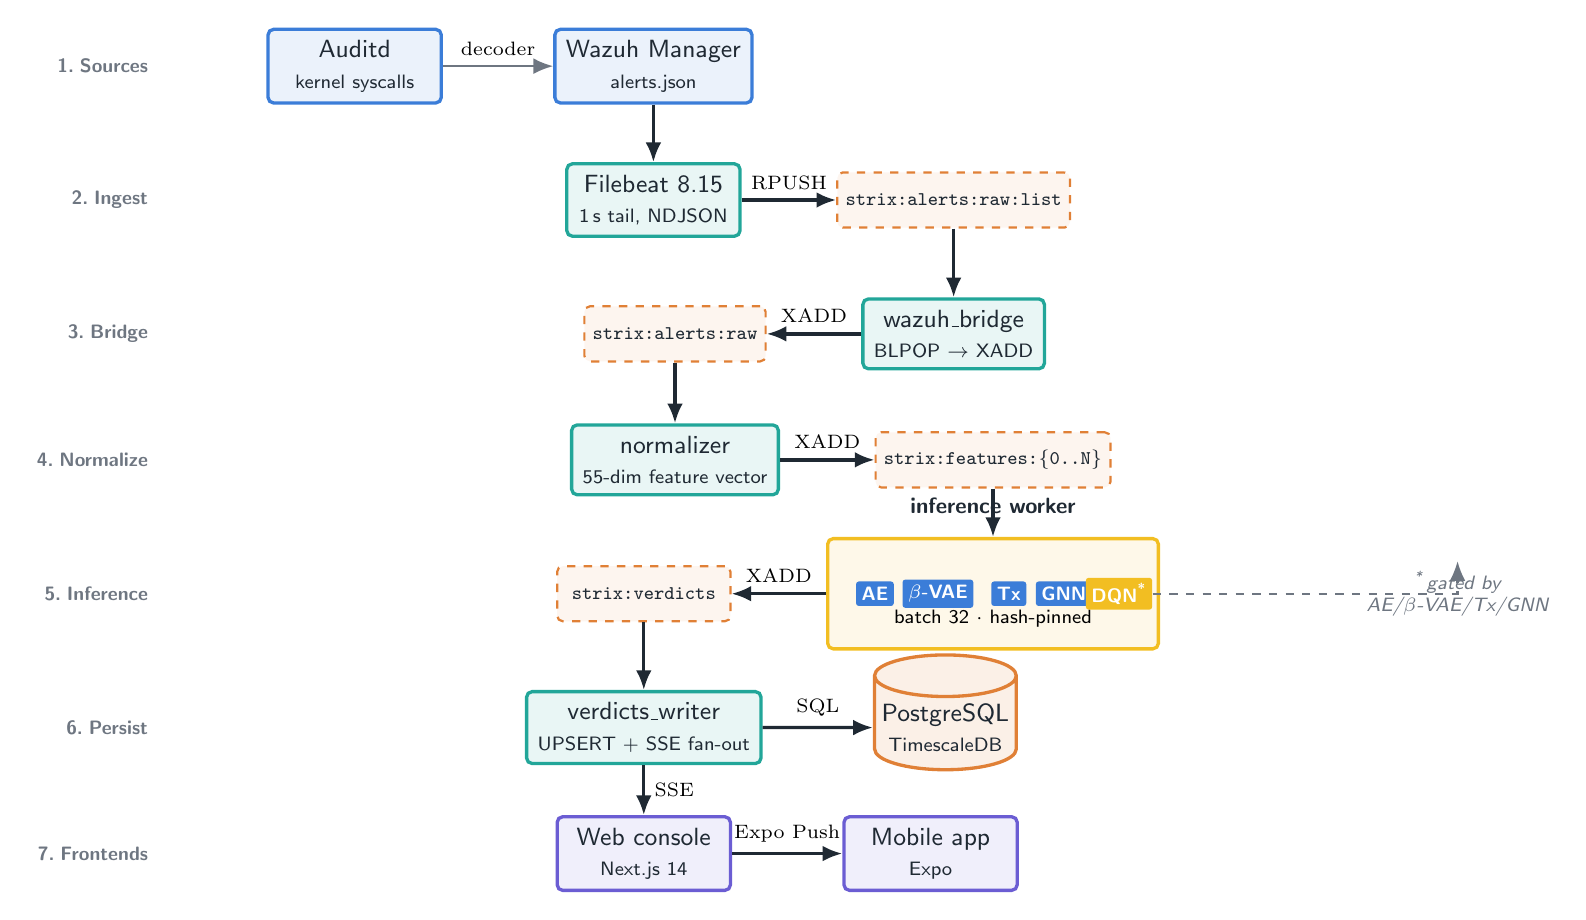
\begin{tikzpicture}[node distance=8mm and 14mm]

% Stage labels on the left
\foreach \y/\lbl in {0/1.\;Sources, -1.7/2.\;Ingest, -3.4/3.\;Bridge, -5.0/4.\;Normalize, -6.7/5.\;Inference, -8.4/6.\;Persist, -10.0/7.\;Frontends}
  \node[anchor=east, font=\sffamily\bfseries\scriptsize, text=strixGrey] at (-1.5,\y) {\lbl};

% ─── Row 1: Sources ──────────────────────────────────────────────
\node[source]                          (auditd) at (1.0, 0)   {Auditd\\\scriptsize kernel syscalls};
\node[source, right=of auditd]         (wazuh)                {Wazuh Manager\\\scriptsize alerts.json};

% ─── Row 2: Filebeat ─────────────────────────────────────────────
\node[worker] (filebeat) at ($(wazuh)+(0,-1.7)$) {Filebeat 8.15\\\scriptsize 1\,s tail, NDJSON};
\node[stream, right=12mm of filebeat] (rlist) {strix:alerts:raw:list};

% ─── Row 3: Bridge ───────────────────────────────────────────────
\node[worker] (bridge) at ($(rlist)+(0,-1.7)$) {wazuh\_bridge\\\scriptsize BLPOP \(\to\) XADD};
\node[stream, left=12mm of bridge] (rraw) {strix:alerts:raw};

% ─── Row 4: Normalizer ───────────────────────────────────────────
\node[worker] (norm) at ($(rraw)+(0,-1.6)$) {normalizer\\\scriptsize 55-dim feature vector};
\node[stream, right=12mm of norm] (rfeat) {strix:features:\{0..N\}};

% ─── Row 5: Inference + 5 models ─────────────────────────────────
\node[model, minimum width=42mm, minimum height=14mm] (inf) at ($(rfeat)+(0,-1.7)$) {};
\node[title, font=\sffamily\bfseries\footnotesize] at ([yshift=4mm]inf.north) {inference worker};
\node[font=\sffamily\scriptsize] at ([yshift=4mm]inf.south) {batch 32 \(\cdot\) hash-pinned};
% Inline model badges
\node[badge=strixBlue] at ([xshift=-15mm,yshift=0mm]inf.center) (mae)  {AE};
\node[badge=strixBlue] at ([xshift=-7mm,yshift=0mm]inf.center) (mvae) {$\beta$-VAE};
\node[badge=strixBlue] at ([xshift=2mm,yshift=0mm]inf.center)  (mtr)  {Tx};
\node[badge=strixBlue] at ([xshift=9mm,yshift=0mm]inf.center)  (mgnn) {GNN};
\node[badge=strixGold] at ([xshift=16mm,yshift=0mm]inf.center) (mdqn) {DQN\textsuperscript{*}};

\node[stream, left=12mm of inf] (rverd) {strix:verdicts};

% ─── Row 6: Persist ──────────────────────────────────────────────
\node[worker] (writer) at ($(rverd)+(0,-1.7)$) {verdicts\_writer\\\scriptsize UPSERT + SSE fan-out};
\node[store, right=14mm of writer] (pg) {PostgreSQL\\\scriptsize TimescaleDB};

% ─── Row 7: Frontends ────────────────────────────────────────────
\node[ui] (web) at ($(writer)+(0,-1.6)$) {Web console\\\scriptsize Next.js 14};
\node[ui, right=14mm of web] (mob) {Mobile app\\\scriptsize Expo};

% ─── Edges ───────────────────────────────────────────────────────
\draw[edge] (auditd) -- (wazuh) node[midway,above,font=\scriptsize] {decoder};
\draw[edgeStrong] (wazuh) -- (filebeat);
\draw[edgeStrong] (filebeat) -- (rlist) node[midway,above,font=\scriptsize] {RPUSH};
\draw[edgeStrong] (rlist) -- (bridge);
\draw[edgeStrong] (bridge) -- (rraw) node[midway,above,font=\scriptsize] {XADD};
\draw[edgeStrong] (rraw) -- (norm);
\draw[edgeStrong] (norm) -- (rfeat) node[midway,above,font=\scriptsize] {XADD};
\draw[edgeStrong] (rfeat) -- (inf);
\draw[edgeStrong] (inf) -- (rverd) node[midway,above,font=\scriptsize] {XADD};
\draw[edgeStrong] (rverd) -- (writer);
\draw[edgeStrong] (writer) -- (pg) node[midway,above,font=\scriptsize] {SQL};
\draw[edgeStrong] (writer) -- (web) node[midway,right,font=\scriptsize] {SSE};
\draw[edgeStrong] (web) -- (mob) node[midway,above,font=\scriptsize] {Expo Push};

% Annotation for the gated DQN
\node[font=\sffamily\scriptsize\itshape, text=strixGrey, anchor=west]
  at ($(inf.east)+(2.5,0)$) (note) {\textsuperscript{*}\,gated by\\AE/$\beta$-VAE/Tx/GNN};
\draw[edge, dashed] (mdqn) -| (note.north);

\end{tikzpicture}
\end{document}
